\documentclass[tikz]{standalone}

\usepackage{amsmath}
\usepackage{circuitikz}

\usetikzlibrary{positioning}

\let\Re\undefined
\let\Im\undefined
\DeclareMathOperator{\Re}{\operatorname{Re}}
\DeclareMathOperator{\Im}{\operatorname{Im}}

\begin{document}
	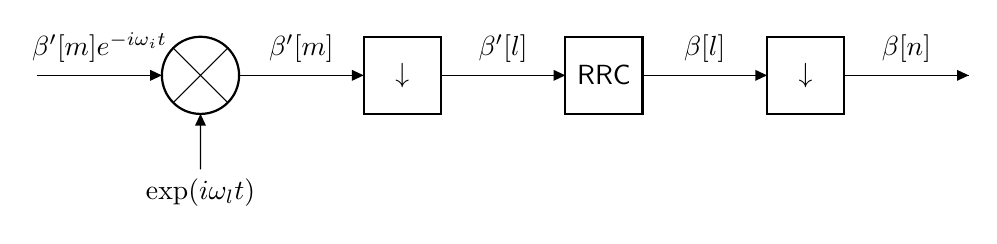
\begin{tikzpicture}[
		node distance=4.5em,
	]
		\coordinate (in) at (0,0);
		\node [mixer, right=of in] (mixer) {};
		\node [twoportshape, t=$\downarrow$, right=of mixer] (dwn1) {};
		\node [twoportshape, t=\sffamily{RRC}, right=of dwn1] (rrc) {};
		\node [twoportshape, t=$\downarrow$, right=of rrc] (dwn2) {};
		\coordinate[right=of dwn2] (out);
		\node [below=2em of mixer] (osc) {$\exp(i\omega_lt)$};
		
		\draw (in) to[short, l={$\beta^\prime[m]e^{-i\omega_it}$}] (mixer.west) node[inputarrow]{};
		\draw (mixer.east) to[short, l={$\beta^\prime[m]$}] (dwn1.west) node[inputarrow]{};
		\draw (dwn1.east) to[short, l={$\beta^\prime[l]$}] (rrc.west) node[inputarrow]{};
		\draw (rrc.east) to[short, l={$\beta[l]$}] (dwn2.west) node[inputarrow]{};
		\draw (dwn2.east) to[short, l={$\beta[n]$}] (out) node[inputarrow]{};
		\draw (osc) to[short] (mixer.south) node[inputarrow, rotate=90]{};
	\end{tikzpicture}
\end{document}
